% =====================================================================
% Course Project Report: Frequent Itemset Mining Using Eclat (Julia)
% Template: HCMUS FIT Report Style (12pt, A4, 1.5 spacing), compiled with XeLaTeX.
% Final PDF submission path: docs/Report.pdf
% =====================================================================
\documentclass[10pt, a4paper]{article}
\usepackage{hcmus}
\usepackage{makecell}
\usepackage{longtable}
\usepackage{tabularx}
\usepackage{titlesec}
\usepackage{enumitem}
\usepackage{tikz}
\usetikzlibrary{positioning, arrows.meta}

\graphicspath{{figures/}}
\singlespacing
\setlist{nosep, leftmargin=*}
\titlespacing*{\section}{0pt}{9pt plus 2pt minus 2pt}{4pt plus 1pt}
\titlespacing*{\subsection}{0pt}{7pt plus 2pt minus 2pt}{3pt plus 1pt}
\titlespacing*{\subsubsection}{0pt}{5pt plus 1pt minus 1pt}{2pt plus 1pt}
\setlength{\textfloatsep}{7pt plus 2pt minus 2pt}
\setlength{\intextsep}{7pt plus 2pt minus 2pt}
\setlength{\floatsep}{6pt plus 2pt minus 2pt}
\setlength{\abovecaptionskip}{4pt}
\setlength{\belowcaptionskip}{2pt}
\renewcommand{\arraystretch}{1.02}

\begin{document}

\begin{titlepage}
\centering


\includegraphics[scale=0.38]{image/hcmus-logo.png}\\[0.5cm]

\textsc{\Large UNIVERSITY OF SCIENCE, VNU-HCM}\\[0.2cm]
\textsc{\Large Faculty of Information Technology}\\[1.2cm]

\textbf{\large CSC14004 -- Data Mining and Applications}\\[0.2cm]
{\normalsize Class: 24KHMT1}\\[1.0cm]

{\Huge \textbf{Course Project Report}}\\[0.35cm]
{\Large Frequent Itemset Mining Using Eclat:\\
Implementation, Performance Evaluation, and Real-World Applications}\\[1.6cm]

\large
\begin{tabular}{rl}
\textbf{Lecturer:} & Prof. Lê Hoài Bắc \\[0.15cm]
\textbf{Lab Instructor:} & M.Sc. Huỳnh Lâm Hải Đăng \\[0.15cm]
\textbf{Teaching Assistant:} & M.Sc. Nguyễn Ngọc Đức
\end{tabular}\\[1.0cm]

\textbf{Students}\\[0.35cm]
\begin{tabular}{ll}
Phạm Trần Anh Quân & \hspace{0.8cm} Student ID: 24127226 \\[0.15cm]
Nguyễn Tiến Cường  & \hspace{0.8cm} Student ID: 24127337
\end{tabular}

\vfill

{\large Semester 1, Academic Year 2026 -- 2027}

\end{titlepage}


\tableofcontents
\newpage

\begin{abstract}
This report presents the from-scratch implementation, verification, experimental evaluation, and real-world applications of the Eclat algorithm for frequent itemset mining in Julia~1.11.4. The implementation adheres to the vertical tidset representation and prefix-based equivalence class decomposition introduced by Zaki~(2000), verified through a three-tier testing framework against a brute-force oracle and the SPMF reference library, and applied to retail market basket analysis and visual pattern discovery.
\end{abstract}

% Giới thiệu (nội dung viết ở mốc M6)
\section{Giới thiệu}
\label{sec:01_gioi_thieu}

Thuật toán Eclat khai thác tập phổ biến (frequent itemset) bằng phép giao tidset.

% II. Kiến thức nền và công trình liên quan (A viết)
\section{Kiến thức nền và công trình liên quan}
\label{sec:nen-tang}

\subsection{Bài toán khai thác tập phổ biến}

Cho tập item $\mathcal{I}$ với $m = |\mathcal{I}|$ và cơ sở dữ liệu (CSDL) giao dịch
$\mathcal{D} = \{T_1, \dots, T_N\}$, trong đó mỗi giao dịch (transaction) $T_j \subseteq \mathcal{I}$ được định danh bởi mã giao dịch (transaction identifier, tid) $j$.
Với một tập item (itemset) $X \subseteq \mathcal{I}$, tập mã giao dịch (tidset) của $X$ là
\begin{equation}
t(X) = \{\, j : X \subseteq T_j \,\},
\label{eq:tidset}
\end{equation}
và độ hỗ trợ (support) của $X$ là $\sigma(X) = |t(X)|$; độ hỗ trợ tương đối là $s(X) = \sigma(X)/N$.
Cho ngưỡng hỗ trợ tối thiểu (minimum support, minsup) $\mathrm{minsup} \in (0, 1]$, đổi sang ngưỡng dạng đếm $\sigma_{\min} = \lceil \mathrm{minsup} \cdot N \rceil$.
Khai thác tập phổ biến (frequent itemset mining, FIM) là liệt kê mọi tập $X \neq \emptyset$ có $\sigma(X) \ge \sigma_{\min}$ cùng support của chúng; ta ký hiệu tập kết quả là $\mathcal{F}$ và $L$ là độ dài giao dịch trung bình.

Không gian tìm kiếm có $2^m - 1$ tập ứng viên, nên mọi thuật toán FIM đều dựa vào tính chất phản đơn điệu (anti-monotone, còn gọi là tính chất Apriori): nếu $X \subseteq Y$ thì $t(Y) \subseteq t(X)$, do đó $\sigma(Y) \le \sigma(X)$; mọi tập con của tập phổ biến đều phổ biến, và mọi tập cha của tập không phổ biến đều không phổ biến.

Từ tập phổ biến có thể sinh luật kết hợp (association rule) $X \Rightarrow Y$ với $X \cap Y = \emptyset$~\cite{agrawal1993mining}:
\begin{equation}
\mathrm{conf}(X \Rightarrow Y) = \frac{\sigma(X \cup Y)}{\sigma(X)}, \qquad
\mathrm{lift}(X \Rightarrow Y) = \frac{\mathrm{conf}(X \Rightarrow Y)}{s(Y)},
\label{eq:rule}
\end{equation}
trong đó độ tin cậy (confidence) là xác suất có $Y$ khi đã có $X$, còn độ nâng (lift) so sánh xác suất đó với xác suất có $Y$ nói chung; $\mathrm{lift} > 1$ nghĩa là $X$ và $Y$ đi cùng nhau nhiều hơn mức ngẫu nhiên~\cite{brin1997dynamic}.

\subsection{Các hướng tiếp cận}

\textbf{Biểu diễn ngang (horizontal layout), duyệt theo mức (level-wise).} Apriori~\cite{agrawal1994fast} sinh ứng viên kích thước $k$ từ các tập phổ biến kích thước $k-1$, cắt tỉa ứng viên có tập con không phổ biến, rồi quét lại CSDL để đếm. Số lần quét bằng độ dài tập phổ biến dài nhất, và số ứng viên có thể bùng nổ ở mức 2.

\textbf{Cây tiền tố.} FP-Growth~\cite{han2000mining} nén CSDL vào một cây tiền tố (FP-tree) sau hai lần quét và khai thác đệ quy trên các cây điều kiện, không sinh ứng viên. Cây nén tốt trên dữ liệu dày nhưng kém trên dữ liệu thưa.

\textbf{Biểu diễn dọc (vertical layout).} Eclat~\cite{zaki2000scalable}, thuật toán được chọn trong đồ án, lưu mỗi item kèm tidset và tính support của tập mới bằng phép giao tidset, không cần quét lại CSDL. Bài báo gốc chia dàn tập con (subset lattice) thành các lớp tương đương theo tiền tố (prefix-based equivalence class) giải độc lập trong bộ nhớ, đề xuất đếm tập 2 item bằng mảng tam giác (triangular array), và cho thấy Eclat thường nhanh hơn Apriori hơn một bậc độ lớn trên dữ liệu tổng hợp (§7). Hai biến thể biểu diễn tidset gắn liền với hướng này: mảng bit (bitset), như thuật toán DLG~\cite{yen1996efficient} dùng một bit-vector cho mỗi item và tính support bằng phép AND; và tập hiệu (diffset) của dEclat~\cite{zaki2003fast}, chỉ lưu phần chênh lệch giữa tidset của tập con và tập cha, rất gọn trên dữ liệu dày.

\textbf{Đánh giá cài đặt.} Hội thảo FIMI'03~\cite{goethals2004advances} chuẩn hóa bộ dữ liệu benchmark (Chess, Mushroom, Retail, Accidents, T10I4D100K) và cho thấy chất lượng cài đặt (cấu trúc dữ liệu, bộ nhớ đệm) ảnh hưởng tới hiệu năng không kém bản thân thuật toán. Thư viện SPMF~\cite{fournier2014spmf} cung cấp cài đặt tham chiếu (reference implementation) bằng Java cho hơn 200 thuật toán; đồ án dùng SPMF như một hộp đen để đối chiếu kết quả và hiệu năng.

\textbf{Ứng dụng.} Phân tích giỏ hàng là ứng dụng kinh điển của luật kết hợp, với bộ dữ liệu Groceries của gói \texttt{arules}~\cite{hahsler2005arules}. Với ảnh, mô hình túi từ thị giác (bag of visual words, BoVW)~\cite{sivic2003video,csurka2004visual} lượng tử hóa bộ mô tả đặc trưng (descriptor) cục bộ, chẳng hạn SIFT~\cite{lowe2004distinctive} hay biểu đồ hướng gradient~\cite{dalal2005histograms}, thành các từ thị giác (visual word) bằng k-means~\cite{arthur2007kmeans}; mỗi ảnh khi đó tương đương một giao dịch. Mẫu nổi bật (emerging pattern)~\cite{dong1999efficient} là các tập phổ biến ở một lớp nhưng hiếm ở lớp khác, đo bằng tỉ lệ tăng $GR_c(X) = s_c(X)/s_{\neg c}(X)$.

% Section 3: Chapter 1 - Implementation
% Division: 3.1, 3.2, 3.4 (Member A - Pham Tran Anh Quan); 3.3, 3.5 (Member B - Nguyen Tien Cuong).
\section{Chapter 1: Implementation}
\label{sec:03_chapter1_implementation}

% ---------------------------------------------------------------------------
\subsection{The Eclat Algorithm from the Original Paper}
\label{subsec:eclat_algo}
% To be completed by Member A (Zaki 2000 §4.1, §4.2, §5.2; Figure F01).

% ---------------------------------------------------------------------------
\subsection{Complexity Analysis}
\label{subsec:complexity}
% To be completed by Member A.

% ---------------------------------------------------------------------------
\subsection{Software Architecture, SPMF I/O, and Command-Line Interface}
\label{subsec:arch_io}

The system is structured as a standalone Julia package, \texttt{EclatFIM} (Julia~1.11.4), partitioned into three isolated dependency environments: a minimal root package (depending solely on \texttt{DataStructures.jl} and the standard library) for the command-line interface and automated test suite; an experimental environment (\texttt{scripts/}) for benchmarking and figure generation; and an application environment for Chapter~3. Figure~\ref{fig:f02_arch} illustrates the modular architecture and end-to-end data flow of the package.

\begin{figure}[H]
\centering
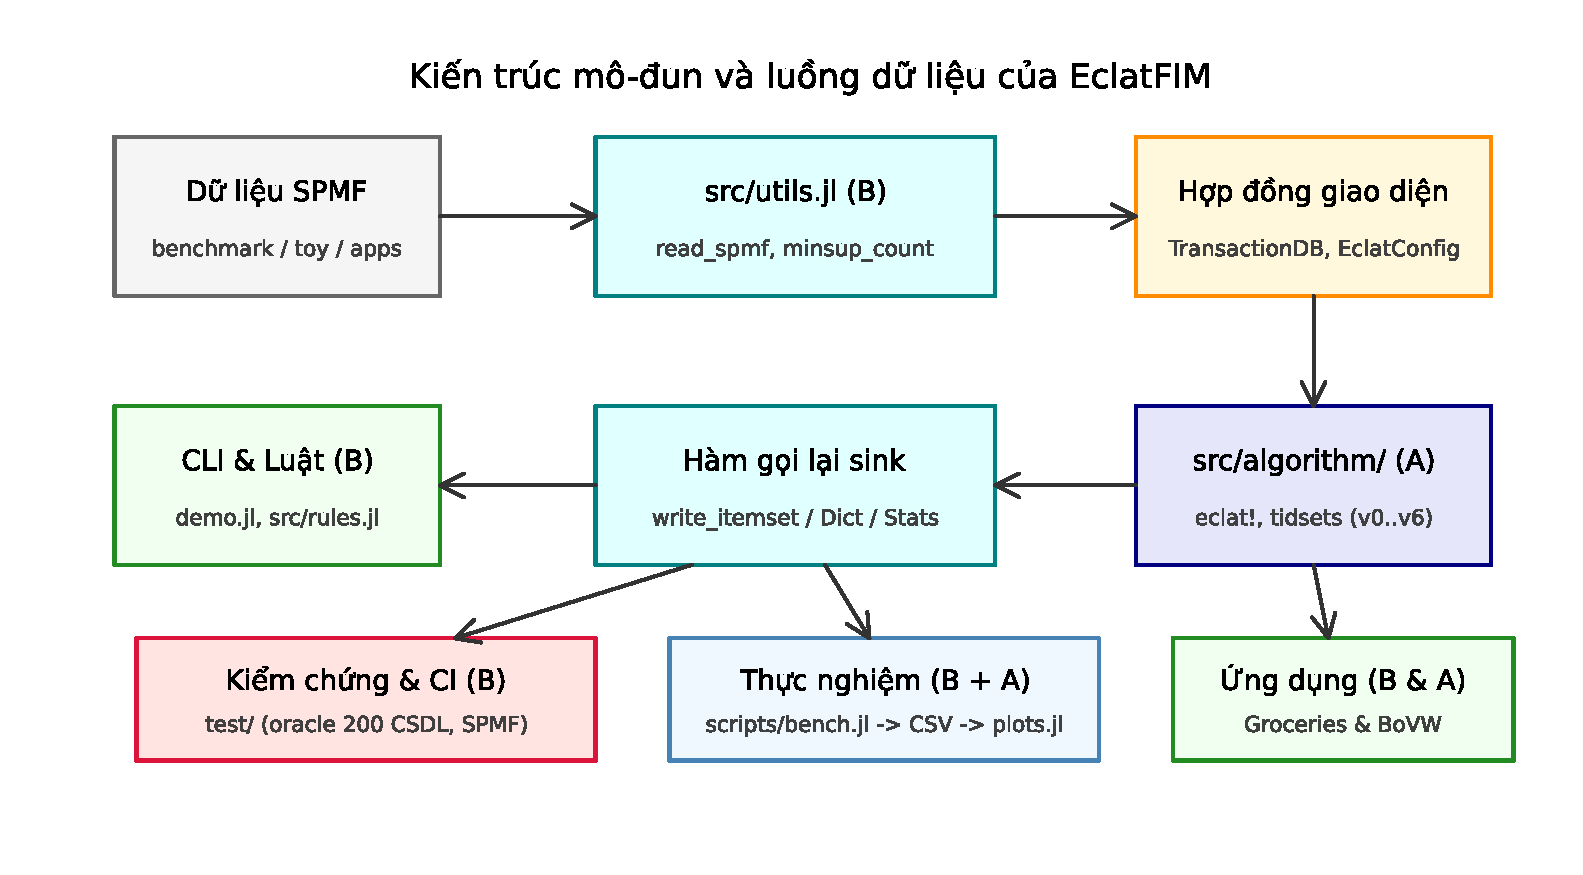
\includegraphics[width=0.92\textwidth]{F02_architecture.pdf}
\caption{Modular architecture and data flow of \texttt{EclatFIM}, separating SPMF-compliant I/O, the interface contract (\texttt{EclatConfig}), the core Eclat mining engine, and downstream verification, benchmarking, and application layers.}
\label{fig:f02_arch}
\end{figure}

The software design centers on three architectural principles:
\begin{enumerate}
    \item \textbf{Decoupled Interface Contract:} The \texttt{TransactionDB} structure maps ascending original item identifiers (\texttt{Int64}) into contiguous internal codes $1 \ldots m$ (\texttt{Int32}), enabling compact array indexing rather than hash-table lookups. The \texttt{EclatConfig} structure decouples independent optimization axes (\texttt{tidset}, \texttt{order}, \texttt{reuse}, \texttt{isect}, \texttt{level2}), allowing a single test suite and benchmarking harness to evaluate every algorithmic variant uniformly without altering call sites.
    \item \textbf{Streaming Output via Callback (\texttt{sink}):} At low minimum support (\texttt{minsup}) thresholds, frequent itemset collections may reach millions of patterns. The core routine \texttt{eclat!(sink, db, minsup, cfg)} emits each frequent itemset through a reusable prefix buffer to \texttt{sink}, allowing direct file streaming without accumulating the entire output set in main memory.
    \item \textbf{Idiomatic Julia Features:} Multiple dispatch specializes tidset intersection operators and eliminates instrumentation overhead at compile time when \texttt{stats === nothing}; generator expressions compute transaction statistics and enumerate proper subsets during rule generation; and \texttt{BinaryMinHeap} and \texttt{counter} from \texttt{DataStructures.jl} extract top-$k$ association rules by lift in $O(n \log k)$ time and tally item frequencies during preprocessing.
\end{enumerate}

To guarantee exact equivalence with the SPMF reference implementation~\cite{fournier2014spmf} (\texttt{spmf.jar}, Eclat v2.65), black-box behavioral experiments were conducted (documented in \texttt{results/spmf\_behavior.md}), establishing two critical I/O conventions:
\begin{itemize}
    \item \emph{Support Threshold Conversion:} SPMF computes the integer support count threshold as $\sigma_{\min} = \lceil \texttt{minsup} \times N \rceil$ using IEEE~754 \texttt{Float64} arithmetic, converting percentage strings \texttt{"p\%"} to $p/100$. Because floating-point rounding can alter boundary outcomes (for example, $0.28 \times 25 = 7.000000000000001$, yielding $\sigma_{\min} = 8$ rather than $7$), \texttt{minsup\_count} reproduces this exact \texttt{Float64} computation to eliminate boundary discrepancies.
    \item \emph{SPMF Parsing and Formatting:} The parser \texttt{read\_spmf} skips empty lines and metadata/comment lines prefixed by \texttt{\#}, \texttt{\%}, or \texttt{@}, and canonicalizes each transaction by sorting and deduplicating items. The writer \texttt{write\_itemset} maps internal codes back to ascending original identifiers, omits the empty itemset, and outputs lines in exact \texttt{i1 i2 ... \#SUP: s} format.
\end{itemize}

The command-line interface \texttt{demo.jl} is implemented without external dependencies and supports \texttt{--minsup} (both ratio and percentage forms), \texttt{-o/--output} (defaulting to \texttt{output.txt}, with \texttt{"-"} streaming patterns to \texttt{stdout} and summary diagnostics to \texttt{stderr}), \texttt{--variant}, and \texttt{--stats}, returning standard exit codes $0$ (success), $1$ (invalid arguments), and $2$ (data or I/O error).

% ---------------------------------------------------------------------------
\subsection{Optimization Techniques}
\label{subsec:optimizations}
% To be completed by Member A (Tables B01, B03, B04 and ablation study v0..v6).

% ---------------------------------------------------------------------------
\subsection{Automated Verification and Match Rate}
\label{subsec:testing}

Correctness is verified independently of the core algorithm author through a three-tier automated testing pipeline located in \texttt{test/}:
\begin{enumerate}
    \item \textbf{Tier 1 — Brute-Force Oracle:} A standalone reference oracle enumerates all $2^m - 1$ non-empty subsets via bitmasks across $200$ randomly generated databases (fixed seeds $1 \ldots 200$, $m \le 12$, $N \le 30$, random $\sigma_{\min}$), verifying $100\%$ exact agreement for every implemented Eclat variant.
    \item \textbf{Tier 2 — Canonical Datasets, Edge Cases, and I/O:} Automated tests validate \texttt{pasquier99.txt} (\texttt{minsup} $= 40\%$, yielding $15$ itemsets) and \texttt{bookstore.txt} from Zaki~\cite{zaki2000scalable} (\texttt{minsup} $= 50\%$, yielding $19$ itemsets, including maximal patterns \texttt{ACTW} and \texttt{CDW}); boundary conditions (empty database, single transaction, identical transactions, \texttt{minsup} $= 100\%$, zero frequent items, large sparse item identifiers); all $10$ floating-point boundary cases of \texttt{minsup\_count}; and hand-verified association rule calculations in \texttt{test\_rules.jl}.
    \item \textbf{Tier 3 — Large-Scale Benchmark Verification:} The comparator \texttt{scripts/compare\_spmf.jl} defines the exact match rate between the implementation's output $\mathcal{F}_{\text{ours}}$ and the SPMF reference output $\mathcal{F}_{\text{SPMF}}$ as:
    \begin{equation}
        \text{Match Rate} = \frac{\left|\{X \in \mathcal{F}_{\text{ours}} \cap \mathcal{F}_{\text{SPMF}} : \sigma_{\text{ours}}(X) = \sigma_{\text{SPMF}}(X)\}\right|}{\left|\mathcal{F}_{\text{ours}} \cup \mathcal{F}_{\text{SPMF}}\right|} \times 100\%.
    \end{equation}
    For outputs exceeding $5 \times 10^6$ itemsets, comparison automatically switches to an order-invariant fingerprint mode: each canonicalized line is hashed with SHA-256, and the leading $64$ bits are accumulated modulo $2^{64}$.
\end{enumerate}

Continuous Integration (GitHub Actions) executes the entire test suite on a clean Julia~1.11.4 environment under both default settings and \texttt{--check-bounds=yes} to verify array-bounds safety for \texttt{@inbounds}-annotated loops. Table~\ref{tab:b02_tests} summarizes the automated verification results across unit tests and four benchmark datasets (\texttt{chess}, \texttt{mushroom}, \texttt{retail}, \texttt{T10I4D100K}).

% Data source: `julia --project=. test/runtests.jl` (commit 52011a2)
\begin{table}[H]
\centering
\caption{Summary of automated test suite execution (\texttt{test/runtests.jl}) for variants \texttt{v0} and \texttt{v1} under default and \texttt{--check-bounds=yes} modes.}
\label{tab:b02_tests}
\begin{tabular}{llrr}
\toprule
Test Group & Source File & Assertions & Pass Rate \\
\midrule
SPMF I/O and \texttt{minsup\_count} & \texttt{test\_io.jl} & 49 & 100\% \\
200-DB brute-force oracle, toy, edge cases & \texttt{test\_correctness.jl} & 62 & 100\% \\
Association rules and \texttt{top\_k} & \texttt{test\_rules.jl} & 225 & 100\% \\
Statistics and cross-variant checks (4 benchmarks) & \texttt{test\_benchmark.jl} & 16 & 100\% \\
\midrule
\textbf{Total} & \texttt{runtests.jl} & \textbf{352} & \textbf{100\%} \\
\bottomrule
\end{tabular}
\end{table}

% Section 4: Chapter 2 - Experiments and Evaluation
\section{Chapter 2: Experiments and Evaluation}
\label{sec:04_chapter2_experiments}

% To be completed after finalizing variants v2..v6 and executing official benchmark runs (E1-E9).

% Section 5: Chapter 3 - Real-World Applications
% Division: 5.1 (Member B - Nguyen Tien Cuong); 5.2 (Member A - Pham Tran Anh Quan).
\section{Chapter 3: Real-World Applications}
\label{sec:05_chapter3_applications}

All frequent itemsets and association rules analyzed in this chapter are mined exclusively using our \texttt{EclatFIM} implementation, without invoking any external frequent itemset mining library.

% ---------------------------------------------------------------------------
\subsection{Application 1: Market Basket Analysis on the Groceries Dataset}
\label{subsec:app1_groceries}

\subsubsection{Problem Formulation and Data Transformation Analysis}
Market basket analysis is conducted on the \texttt{Groceries} retail dataset from the \texttt{arules} package~\cite{hahsler2005arules}, comprising $N = 9{,}835$ point-of-sale transactions across $m = 169$ named product items. Unlike anonymized datasets such as \texttt{Retail}, explicit product names in \texttt{Groceries} allow direct domain interpretation. Each receipt is converted into an SPMF-formatted transaction accompanied by \texttt{@ITEM=id=name} metadata lines; \texttt{read\_spmf} ignores metadata directives during mining and maps item codes back to product names for rule interpretation.

To evaluate how transaction granularity affects Eclat's behavior, two transformation schemes are compared at $\texttt{minsup} = 1\%$ ($\sigma_{\min} = 99$) and $\texttt{minconf} = 0.3$: (i) retaining all $169$ fine-grained product items, and (ii) aggregating items into $12$ coarse supermarket categories (such as \texttt{dairy\_eggs}, \texttt{produce}, \texttt{bakery}, and \texttt{meat\_seafood}). Table~\ref{tab:b08_groceries_transform} highlights two key findings:
\begin{itemize}
    \item Under the fine-grained $169$-item representation, the average density is $\rho = \bar{L}/m = 2.61\%$, closely approaching the theoretical $1/32 \approx 3.125\%$ crossover threshold between \texttt{Vector\{Int32\}} and \texttt{BitVector} tidset representations in Eclat. With short transactions ($\bar{L} = 4.41$), mining completes in $0.0256$~s and yields $125$ actionable rules.
    \item Aggregating into $12$ coarse categories increases density nearly tenfold to $25.98\%$, expanding the pattern space from $333$ to $477$ frequent itemsets and causing rule volume to surge to $2{,}232$ overly generic rules (e.g., \emph{dairy $\Rightarrow$ produce}) that offer limited merchandising utility. Consequently, the $169$-item representation is selected.
\end{itemize}

% Data source: results/groceries_b08_transforms.csv
\begin{table}[H]
\centering
\caption{Quantitative comparison of two Groceries transformation schemes at $\texttt{minsup} = 1\%$, $\texttt{minconf} = 0.3$ (variant \texttt{v1}).}
\label{tab:b08_groceries_transform}
\begin{tabular}{lrrrrrr}
\toprule
Representation Scheme & $m$ & $\bar{L}$ & $\rho$ & $|\mathcal{F}|$ & Rules & Runtime \\
\midrule
169 original items (selected) & 169 & 4.41 & 2.61\% & 333 & 125 & 0.0256 s \\
12 coarse product categories & 12 & 3.12 & 25.98\% & 477 & 2,232 & 0.0024 s \\
\bottomrule
\end{tabular}
\end{table}

\subsubsection{Threshold Sensitivity Analysis}
Rule sensitivity is evaluated over the parameter grid $\texttt{minsup} \in \{0.5\%, 1\%, 2\%\} \times \texttt{minconf} \in \{0.2, 0.3, 0.5\}$ (\texttt{results/groceries\_grid.csv}). At $\texttt{minsup} = 0.5\%$ ($\sigma_{\min} = 50$), the algorithm produces $1{,}001$ frequent itemsets and up to $893$ rules (at $\texttt{minconf} = 0.2$), introducing numerous low-evidence associations. Conversely, at $\texttt{minsup} = 2\%$ ($\sigma_{\min} = 197$), only $37$ rules remain at $\texttt{minconf} = 0.3$ (and a single rule at $0.5$), pruning specialized purchasing patterns. Selecting $\texttt{minsup} = 1\%$ ($\sigma_{\min} = 99$) and $\texttt{minconf} = 0.3$ yields $125$ rules, striking a balanced trade-off between coverage and interpretability.

\subsubsection{Primary Results and Business Interpretation}
Figure~\ref{fig:f11_groceries} maps all $125$ rules across support and confidence, color-coded by lift. Ranking by confidence alone exhibits strong popularity bias: \texttt{whole milk} appears in $2{,}513/9{,}835$ baskets ($25.55\%$), causing top-confidence rules to predominantly feature \texttt{whole milk} as the consequent despite modest lift (e.g., \texttt{curd + yogurt} $\Rightarrow$ \texttt{whole milk} achieves $\text{conf} = 0.582$ with $\text{lift} = 2.279$). Ranking by lift~\cite{brin1997dynamic} adjusts for baseline prevalence and surfaces genuine co-purchasing affinities (Table~\ref{tab:b09_groceries_top10}).

\begin{figure}[H]
\centering
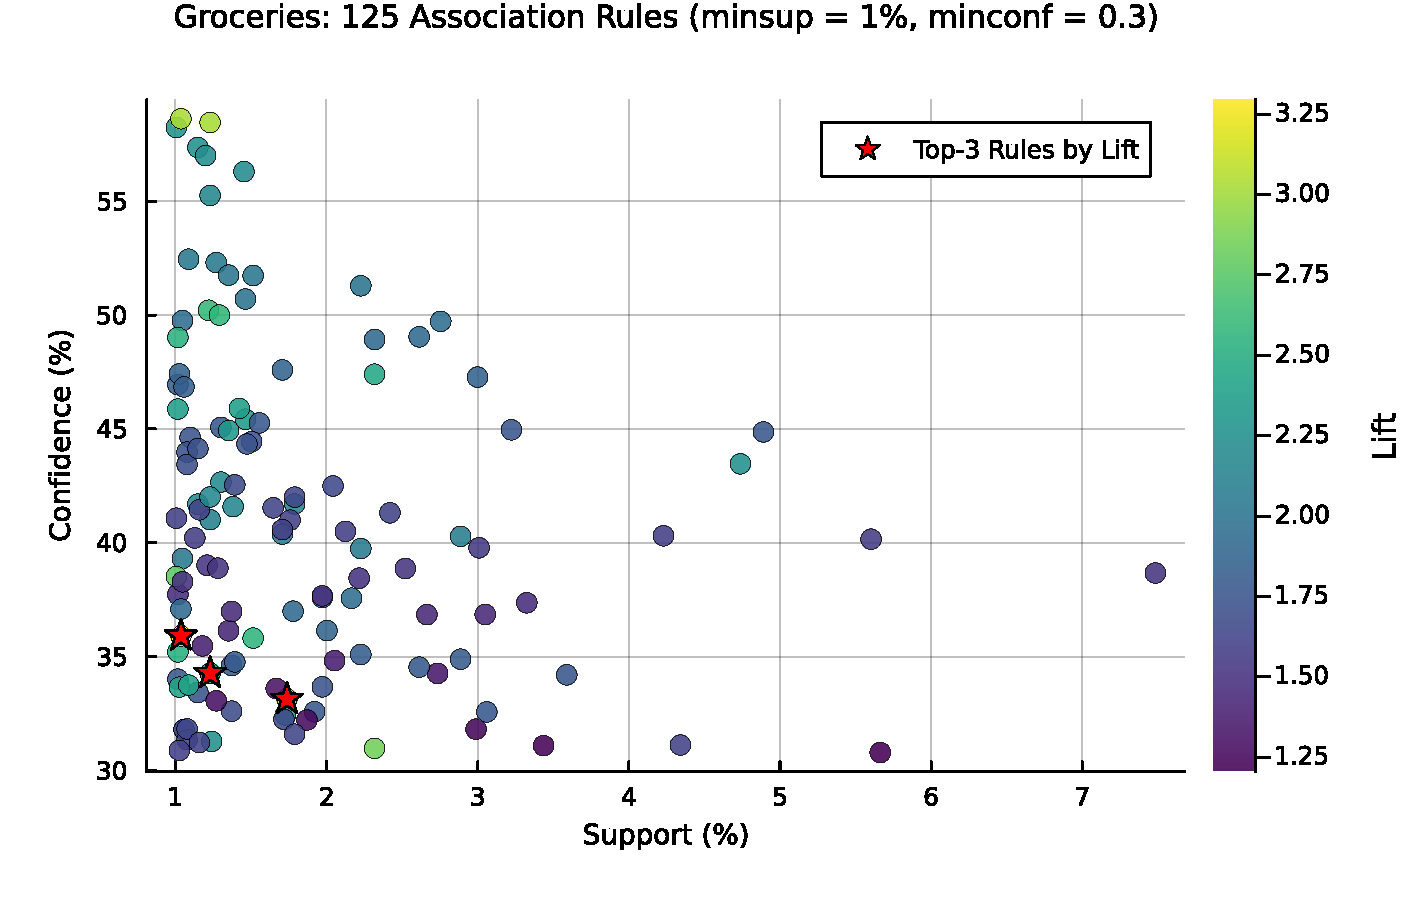
\includegraphics[width=0.88\textwidth]{F11_groceries_rules.pdf}
\caption{Distribution of $125$ association rules on the Groceries dataset ($\texttt{minsup} = 1\%$, $\texttt{minconf} = 0.3$) across support and confidence, colored by lift; red stars denote the top-3 rules by lift.}
\label{fig:f11_groceries}
\end{figure}

% Data source: results/groceries_top10.csv
\begin{table}[H]
\centering
\caption{Top-10 association rules ranked by lift on the Groceries dataset ($\texttt{minsup} = 1\%$, $\texttt{minconf} = 0.3$).}
\label{tab:b09_groceries_top10}
\begin{tabular}{rllrrrr}
\toprule
Rank & Antecedent ($X$) & Consequent ($Y$) & $\sigma$ & Support & Confidence & Lift \\
\midrule
1 & citrus fruit + other vegetables & root vegetables & 102 & 0.0104 & 0.3592 & 3.295 \\
2 & other vegetables + tropical fruit & root vegetables & 121 & 0.0123 & 0.3428 & 3.145 \\
3 & beef & root vegetables & 171 & 0.0174 & 0.3314 & 3.040 \\
4 & citrus fruit + root vegetables & other vegetables & 102 & 0.0104 & 0.5862 & 3.030 \\
5 & root vegetables + tropical fruit & other vegetables & 121 & 0.0123 & 0.5845 & 3.021 \\
6 & other vegetables + whole milk & root vegetables & 228 & 0.0232 & 0.3098 & 2.842 \\
7 & curd + whole milk & yogurt & 99 & 0.0101 & 0.3852 & 2.761 \\
8 & rolls/buns + root vegetables & other vegetables & 120 & 0.0122 & 0.5021 & 2.595 \\
9 & root vegetables + yogurt & other vegetables & 127 & 0.0129 & 0.5000 & 2.584 \\
10 & tropical fruit + whole milk & yogurt & 149 & 0.0151 & 0.3582 & 2.568 \\
\bottomrule
\end{tabular}
\end{table}

The top rules in Table~\ref{tab:b09_groceries_top10} reveal three actionable consumer clusters:
\begin{itemize}
    \item \textbf{Home-Cooking Ingredients (Rank~3):} Customers purchasing \texttt{beef} buy \texttt{root vegetables} at $3.04\times$ the baseline rate ($\sigma = 171$), reflecting meal-preparation habits (e.g., stews and soups). Placing fresh root vegetables adjacent to the meat counter or offering bundled meal kits directly leverages this affinity.
    \item \textbf{Fresh Produce Cluster (Ranks~1, 2, 4, 5):} \texttt{citrus fruit}, \texttt{tropical fruit}, \texttt{other vegetables}, and \texttt{root vegetables} exhibit strong mutual reinforcement ($\text{lift} > 3.0$), supporting contiguous produce layouts and multi-item produce promotions.
    \item \textbf{Dairy Cluster (Ranks~7, 10):} \texttt{curd + whole milk} $\Rightarrow$ \texttt{yogurt} ($\text{lift} = 2.761$) supports cross-promotional placement within refrigerated dairy aisles.
\end{itemize}

\subsubsection{Out-of-Sample Stability Evaluation (80/20 Split)}
Rule generalizability is assessed via a reproducible $80\%/20\%$ random split (\texttt{seed} $= 42$), yielding $N_{\text{train}} = 7{,}868$ training baskets and $N_{\text{test}} = 1{,}967$ test baskets. The top-10 rules by lift mined on the training split are re-evaluated on the held-out test split (Table~\ref{tab:b10_groceries_stability}). All $10/10$ rules preserve $\text{test\_lift} > 1.5$. Core associations such as Rank~1 ($-4.5\%$ shift), Rank~5 ($-3.4\%$), and Rank~4 (\texttt{beef} $\Rightarrow$ \texttt{root vegetables}, $-8.5\%$) demonstrate high stability, whereas Rank~6 (\texttt{whipped/sour cream + whole milk} $\Rightarrow$ \texttt{root vegetables}) experiences a $-38.3\%$ drop due to higher sampling variance near the $1\%$ support boundary.

% Data source: results/groceries_stability.csv
\begin{table}[H]
\centering
\caption{Stability evaluation of top-10 training rules by lift on an $80/20$ split (\texttt{seed} $= 42$, $N_{\text{train}} = 7{,}868$, $N_{\text{test}} = 1{,}967$).}
\label{tab:b10_groceries_stability}
\begin{tabular}{rlrrr}
\toprule
Rank & Rule ($X \Rightarrow Y$) & Train Lift & Test Lift & Shift \\
\midrule
1 & citrus fruit + other vegetables $\Rightarrow$ root vegetables & 3.325 & 3.175 & $-4.5\%$ \\
2 & other vegetables + tropical fruit $\Rightarrow$ root vegetables & 3.242 & 2.734 & $-15.7\%$ \\
3 & citrus fruit + root vegetables $\Rightarrow$ other vegetables & 3.159 & 2.568 & $-18.7\%$ \\
4 & beef $\Rightarrow$ root vegetables & 3.093 & 2.831 & $-8.5\%$ \\
5 & root vegetables + tropical fruit $\Rightarrow$ other vegetables & 3.040 & 2.935 & $-3.4\%$ \\
6 & whipped/sour cream + whole milk $\Rightarrow$ root vegetables & 2.925 & 1.805 & $-38.3\%$ \\
7 & other vegetables + yogurt $\Rightarrow$ root vegetables & 2.864 & 2.203 & $-23.1\%$ \\
8 & other vegetables + whole milk $\Rightarrow$ root vegetables & 2.787 & 3.072 & $+10.2\%$ \\
9 & other vegetables + whipped/sour cream $\Rightarrow$ yogurt & 2.612 & 2.214 & $-15.3\%$ \\
10 & rolls/buns + root vegetables $\Rightarrow$ other vegetables & 2.588 & 2.628 & $+1.5\%$ \\
\bottomrule
\end{tabular}
\end{table}

\subsubsection{Limitations and Practical Extensions}
Three methodological limitations warrant caution when operationalizing association rules: (i) high-lift rules with support near the minimum threshold rest on limited sample evidence and exhibit higher out-of-sample variance; (ii) lift is symmetric ($\text{lift}(X \Rightarrow Y) = \text{lift}(Y \Rightarrow X)$) and therefore does not identify purchase directionality; and (iii) co-occurrence does not imply causality, as unobserved confounders such as weekend shopping cycles or seasonality may drive joint demand. In practice, stable rules can feed real-time e-commerce basket recommenders or generate hypotheses for controlled A/B shelf-placement experiments.

% ---------------------------------------------------------------------------
\subsection{Application 2: Visual Pattern Discovery via Bag of Visual Words}
\label{subsec:app2_bovw}
% To be completed by Member A (Caltech-101, Tables B11-B13, Figures F12-F13).

% VI. Kết luận và hướng phát triển — cả hai cùng viết.
\section{Kết luận và hướng phát triển}
\label{sec:ket-luan}

Nhóm đã cài đặt lại Eclat từ bài báo gốc bằng Julia, với bảy phiên bản cho phép đo riêng tác dụng của từng tối ưu. Về tính đúng, cả 245 tổ hợp (bộ dữ liệu, minsup, phiên bản) khớp SPMF 100\%, cùng 15.869 phép kiểm tra tự động trên ba tầng độc lập. Về hiệu năng, bản mặc định nhanh hơn SPMF \texttt{Eclat} ở mọi mức minsup và nhanh hơn \texttt{Eclat\_bitset} ở 34/35 mức, xét theo thời gian thuật toán; điểm yếu chính là 4,5--6 giây khởi động của Julia. Hai ứng dụng đều chạy bằng chính cài đặt của nhóm. Trên Groceries, các luật theo lift cho thấy hai hành vi mua rõ ràng và ổn định khi kiểm tra trên dữ liệu giữ lại. Trên ảnh, các mẫu trực quan phản ánh cấu trúc hình học của từng lớp, làm lộ thiên lệch phông nền của lớp khuôn mặt, và đạt 75,8\% độ chính xác khi dùng làm đặc trưng.

Đối chiếu dự đoán với số đo là phần nhóm học được nhiều nhất. Các giả thuyết về tính đúng (H1), thứ tự item (H3), khả năng mở rộng (H4), độ dài giao dịch (H5) và ưu thế so với Apriori, FP-Growth (H6) được xác nhận; riêng H6 còn cho thấy SPMF \texttt{Apriori} nhanh hơn chính SPMF \texttt{Eclat} ở 22/33 mức, tức chất lượng cài đặt quan trọng không kém thuật toán. Một số dự đoán chỉ đúng một phần hoặc sai, và mỗi chỗ lệch đều giải thích được bằng số đo: mảng bit nhanh hơn mảng chỉ số ở mật độ thấp hơn nhiều so với ngưỡng bộ nhớ $1/32$, trừ khi hầu hết phép giao thất bại (H2); mảng tam giác có hại khi $N$ rất lớn mà ít item phổ biến (H8); bộ nhớ không có đỉnh ở mức 2 vì cách duyệt sâu của nhóm khác cách duyệt của bài báo (H7). Vì vậy không có một phiên bản nào nhanh nhất trên mọi dữ liệu.

Hướng phát triển, theo thứ tự lợi ích dự kiến: chọn biểu diễn tidset bằng mô hình chi phí thời gian, dùng số đếm sẵn có của mảng tam giác; giảm thời gian khởi động bằng PrecompileTools.jl; dùng diffset cho dữ liệu dày; song song hóa các lớp ở mức 1. Cùng khung lớp tiền tố này, bài báo còn đề xuất MaxEclat và MaxClique để tìm nhanh các tập phổ biến tối đại dài; đây là bước mở rộng tự nhiên tiếp theo.


\newpage
\bibliographystyle{IEEEtran}
\bibliography{references}

\newpage
\appendix
% Appendix
\section{Supplementary Tables and Reproducibility Notes}
\label{sec:07_appendix}

% ---------------------------------------------------------------------------
\subsection{Reproducing Every Result}
\label{subsec:appendix_reproduce}

Every number in this report is produced by a script in the repository and stored as a CSV or Markdown file in \texttt{results/}; every run appends the command, commit, and duration to \texttt{results/LOG.md}. All random choices use the fixed seed $42$ (synthetic data, subsampling, image selection, $k$-means). Table~\ref{tab:appendix_commands} maps each result to the command that regenerates it; the notebook \texttt{notebooks/demo.ipynb} runs the same commands on Google Colab.

\begin{table}[H]
\centering
\caption{Commands that regenerate the results of the report (run from the repository root).}
\label{tab:appendix_commands}
\begin{tabular}{@{}p{3.6cm}p{12.0cm}@{}}
\toprule
Result & Command \\
\midrule
Test suite (Table~\ref{tab:b02_tests}) & \texttt{julia --project=. test/runtests.jl} \\
E1--E6, E9 & \texttt{julia --project=. scripts/run\_chapter2.jl --only e2} (and \texttt{e5}, \texttt{e6}, \texttt{e9}) \\
E8 (Tables~\ref{tab:b03_ablation_time}, \ref{tab:b04_ablation_counters}) & \texttt{julia --project=. scripts/bench\_ablation.jl} \\
E7 (Figure~\ref{fig:f08_density}) & \texttt{julia --project=. scripts/bench\_density.jl} \\
E10 (Figure~\ref{fig:f10_memory_trace}) & \texttt{julia --project=. scripts/bench\_memory\_trace.jl} \\
Figures F08, F10 & \texttt{julia --project=apps scripts/plots\_a.jl} \\
Application 1 & \texttt{julia --project=. apps/groceries/run\_groceries.jl} \\
Application 2 & \texttt{julia --project=apps apps/bovw/prepare.jl}, then \texttt{analyze.jl}, \texttt{figures.jl} \\
\bottomrule
\end{tabular}
\end{table}

\textbf{Measurement machines.} Experiments E1--E6 and E9 were run on the reference machine described in Section~\ref{subsec:exp_setup} (\texttt{results/ENV.md}). Experiments E7, E8, E10 and Application~2 were run on a second machine (\texttt{results/ENV\_A.md}): Intel Core i5-6200U (2.30~GHz, 4 hardware threads, 10.1~GiB RAM, Windows~x64), Julia~1.11.4 single-threaded. Absolute times are therefore not comparable between E2 and E8; every comparison in this report is made between measurements taken on the same machine, under the same protocol (fresh process, warm-up on a toy dataset, \texttt{time\_ns()}, median of 3 runs or 5 runs below one second, counters collected in a separate untimed run).

% ---------------------------------------------------------------------------
\subsection{Libraries Used Outside the Mining Algorithm}
\label{subsec:appendix_libraries}

The mining algorithm (\texttt{src/}) depends only on the Julia standard library and \texttt{DataStructures.jl} (\texttt{BinaryMinHeap} for top-$k$ rules). The experiment and application environments use additional libraries for purposes unrelated to frequent itemset mining:

\begin{table}[H]
\centering
\caption{Libraries outside the mining algorithm and their purpose.}
\label{tab:appendix_libraries}
\begin{tabular}{@{}lll@{}}
\toprule
Library & Environment & Purpose \\
\midrule
\texttt{CSV.jl}, \texttt{DataFrames.jl}, \texttt{Plots.jl} & \texttt{scripts/} & reading result tables and drawing the Chapter~2 figures \\
\texttt{JpegTurbo.jl} & \texttt{apps/} & decoding Caltech-101 JPEG images \\
\texttt{ColorTypes.jl} & \texttt{apps/} & converting RGB pixels to grayscale \\
\texttt{Plots.jl} & \texttt{apps/} & Figures F08, F10, F12, F13 \\
\texttt{LinearAlgebra}, \texttt{Statistics}, \texttt{Random} & standard library & distances in $k$-means, standardization, seeded sampling \\
\bottomrule
\end{tabular}
\end{table}

No external frequent itemset mining, clustering, or classification library is used: $k$-means++, the gradient-orientation descriptors, and the logistic regression classifier of Application~2 are implemented in \texttt{apps/bovw/}.


\end{document}
